%!TEX root = ../dokumentation.tex

\chapter{Rahmenbedinungnen}

\section{Programmiersprache}

\section{Webserver}

Ein Webserver ist in der Regel ein Server, der zur Verbreitung von Webinhalten im Inter- oder Intranet dient. Die jeweiligen Informationen und Dokumentationen können demnach weltweit oder firmenintern erreicht werden. Damit eine Website jederzeit erreichbar sein kann, muss der Webserver permanent online sein.
Der Rechner, auf dem der Webserver läuft, wird als Host bezeichnet. Der Webserver ist für die zuverlässige Übertragung von statischen, wie beispielsweise von unveränderlichen \ac{HTML}-Dateien, aber auch von dynamischen Dateien verantwortlich. Für dynamische Dateien muss der Webserver vor der Antwort Programmcode ausführen. Dieser Programmcode wird in diesem Fall in der Programmiersprache Python geschrieben. Mittels einer \ac{CSS} Datei können die Inhalte der dynamischen Dateien weitestgehend von den Darstellungsvorgaben getrennt werden. In der \ac{HTML} Datei wird folglich nur die inhaltliche Gliederung definiert und in der \ac{CSS} Datei die Darstellung, wie etwa Farben oder Layout.
Für die Übermittlung wird das Übertragungsprotokoll \ac{HTTP} oder die verschlüsselte Variante \ac{HTTPS} verwendet.
Ein Webserver ist in der Lage, die Inhalte auf viele verschiedene Rechner gleichzeitig zu übermitteln. Wie viele Nutzeranfragen (Requests) ein Server bearbeiten kann, hängt von der Hardware und der Auslastung des Hosts ab.

\begin{figure}[htbp]
	\centering
	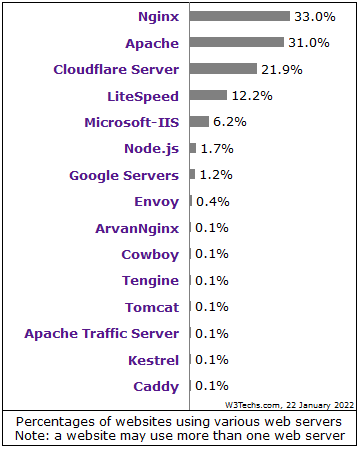
\includegraphics{images/StatistikWebserver.png}
	\caption{Quelle: https://w3techs.com/technologies/overview/web\_server}
	\label{fig:WebserverStatistik}
\end{figure}


Am verbreiteten sind unter anderem die Webserver Computerprogramme Apache HTTP Server und nginx wie in die Statistik \ref{fig:WebserverStatistik}. Beide Programme sind freie Software und wurden daher für das Projekt in Betracht gezogen. Im Folgenden werden diese beide Programme verglichen.


\subsection{Apache HTTP Server}

Der Apache Webserver wurde erstmals 1195 veröffentlicht und hat sich schnell zu einem der beliebtesten Webserver entwickelt. Er unterstützt neben Unix und Linux noch eine Vielzahl an weiteren Betriebssystemen.

Beim Apache-Webserver wird ein Ansatz verfolgt, bei dem jede Clientanfrage von einem separaten Prozess oder Thread bearbeitet wird. Dadurch werden Prozesse, die Schreib- oder Leseoperationen erfordern, nacheinander abgearbeitet und es kann passieren, dass ein Request in der Warteschlange verweilen muss, bis der vorherige Request durchgeführt werden konnte. Damit man dieses Problem umgehen kann, gibt es die Möglichkeit mehrere Single-Threading-Prozesse gleichzeitig zu starten. Diese Strategie ist jedoch mit einem hohen Ressourcenaufwand verbunden. Um dies zu vermeiden, kommen Multi-Threading-Mechanismen zum Einsatz. Für die parallele Abfrage von Clientanfragen gibt es verschiedene Multi-Processing-Module, die integriert werden können.

Der Apache Server ist modular aufgebaut, wodurch benötigte Funktionen, die der Server nicht nativ bereitstellt, durch Module importiert werden können. Das Erstellen dynamischer Webseiten wird mittels serverseitiger Skriptsprachen bewerkstelligt. Über ein Modul kann der entsprechende Interpreter in den Server integriert werden.


\subsection{Nginx Webserver}

Der Marktanteil von Nginx ist in den letzten Jahren kontinuierlich gestiegen, weshalb auch dieser Webserver für die Studienarbeit in Betracht gezogen wurde. Nginx wurde erstmals 2004 veröffentlicht und ist wie der Apache Server auch mit diversen Betriebssystemen kompatibel.

Dieser Server zeichnet sich durch eine hohe Performance aus. Dabei können eine möglichst große Anzahl an Clients gleichzeitig bedient werden und der Ressourcenverbrauch trotzdem gering gehalten. Durch die ereignisorientierte Architektur können Client-Anfragen asynchron bearbeitet werden, wodurch Arbeitsspeicher und Zeit gespart werden kann. Die Nebenläufigkeit ist realisiert, ohne dass für jede neue Verbindung ein zusätzlicher Prozess oder Thread benötigt wird.  Die Stärke dieser Architektur zeigt sich bei großen Webprojekten.

Wie Apache ist auch Nginx modular aufgebaut und verschiedene Funktionen können über Module bereitgestellt werden. Zu diesen Modulen gehört jedoch nicht die Option Interpreter für eine Programmiersprache entsprechend in den Webserver zu integrieren. Es wird also ein weiterer Anwendungsserver benötigt. Für kleine Webprojekte ist das ein Mehraufwand, der nicht immer eingegangen werden muss. 


\subsection{Fazit}

Die folgende Tabelle \ref{tab:ServerVergleich} zeigt die Unterschiede und Gemeinsamkeiten der beiden Webserver auf. Der ausschlaggebende Grund warum sich für einen Apache Server entschieden wurde, ist das Merkmal der dynamischen Webinhalte.

\newlength{\colWidth}
\setlength{\colWidth}{0.33\textwidth}
\begin{table}[htbp]
	\centering
	\begin{tabular}{p{\colWidth}p{\colWidth} p{\colWidth}}
		\hline
		Merkmal & Apache & NGINX \\
		\hline
		Funktion & Webserver, Proxy-Server & Webserver, Proxy-Server, E-Mail-Proxy, Load-Balancer \\
		Betriebssystem & Alle unixoiden Plattformen, Windows & FreeBSD, Linux, Solaris, IBM AIX, HP-UX, macOS, Windows \\
		Lizenz & Apache License v2.0 & \acs{BSD}-Lizenz \\
		Entwickler & Apache Software Foundation & Nginx, Inc. \\
		Statische Webinhalte & Ja & Ja \\
		Dynamische Webinhalte & Ja & Nein \\
		Software-Architektur & Prozess-/threadbasiert & Eventgesteuert \\
		\hline
	\end{tabular}
	\caption[Tabelle]{Vergleich der Webserver Apache HTTP Server und Nginx Webserver}
	\label{tab:ServerVergleich}
\end{table}

Der Apache Webserver bietet eine breite Möglichkeit an Modulen, um die Software zu erweitern.
Der ausschlaggebende Grund, warum sich in diesem Projekt für den Apache HTTP Server entschieden wurde, ist die Möglichkeit Interpreter für Programmiersprachen über ein Modul direkt in den Webserver zu integrieren. Zudem muss für das Projekt nur ein Client bedient werden. Dadurch wird für das Anzeigen von dynamischen Inhalten kein separaten  Anwendungsserver benötigt. Dadurch bietet der Apache HTTP Server eine bequemere Lösung für kleine Websites, deren Inhalt dynamisch erzeugt wird.





\section{Framework}

\subsection{Django}

\subsection{Flask}



\section{Entwurfsmuster}

\subsection{MVC}